\section{Workflow re-engineering}

Reorganizing the work flow has been the most time-consuming activity in
this part of the project, especially since in our case automation and
integration are the keys. In order to avoid to change the work flow during
the process of building the CI we spent a large amount of time trying to
modularize and split every jobs in all his components.

The main use cases that we identified is for testing CRM tickets: as
explained in the previous sections, every time a new change in the
configuration manifests is submitted, the CI needs to test that a build
with that change is not failing. Some tests are provided in order to
identify issues.
  
\subsection{Adding the tests}

Since, as explained before, one of the keys of our project needs to be
automation we decided to create a Jenkins job called
\textit{setup-base-tests} in order to add sample tests to the user's
module. This job configures the user module with some sample tests and
adds to Jenkins a new job dedicated to that specific module.

For the final user setting up the tests becomes as simple as opening
a normal CRM ticket: the user opens a ticket with Jira type \textit{Add
test templates} and specifies the module name. The Configuration Team then
reviews the request and, if the user is authorized to use the CI service,
moves the ticket from \textit{Pending} to \textit{Approved}. This
operation triggers a Jira webhook that starts a Jenkins job called
\textit{setup-base-tests}.

\begin{figure}[H]
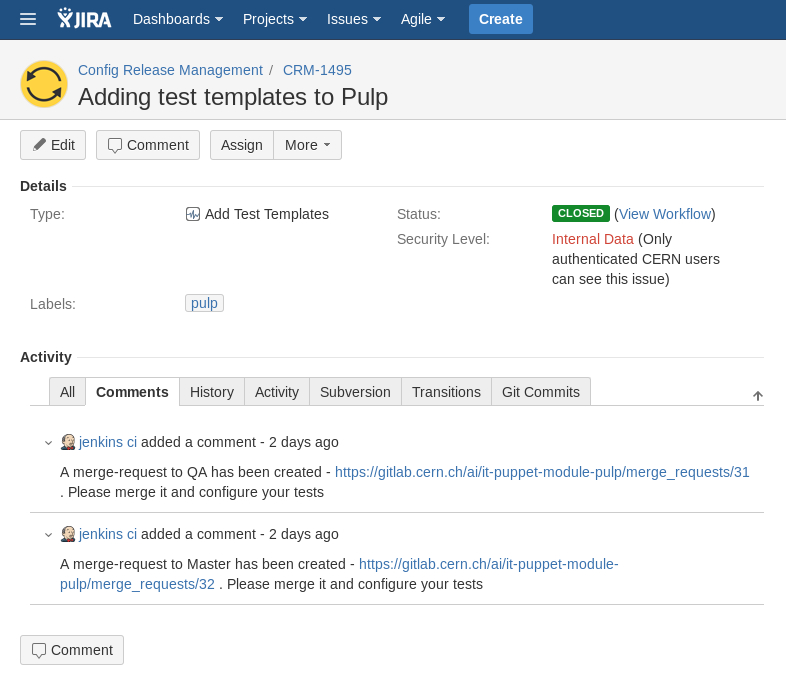
\includegraphics[width=\textwidth,height=\textheight,keepaspectratio]{ContinuousIntegrationWithJenkins/images/add_test_templates.jpg}
\caption{JIRA ticket to add test templates}
\end{figure}

This job scans Jira for tickets with type \textit{Add test templates} and
status \textit{Approved} and gets the module name from them. Then, it
clones the corresponding git repository of the module and, in a new branch
called \textit{add-tests} adds a folder containing all the test samples.
If all the operations are completed successfully, it creates two merge
requests on Gitlab: one from \textit{add-tests} to \textit{qa} and one to
\textit{master}. These requests need to be approved by the service manager
responsible for the module.

Following this, a new Jenkins jobs with the name of the module is created
(that will be triggered when a new CRM ticket is opened) and, if
everything goes well, the original Jira ticket is closed with status
\textit{Completed}.

At this point the user can customize the tests and the Puppet manifests
that are present inside the module's repository merging the test samples
inside the repository and then editing them accordingly. 

\subsection{Proposing a configuration change}

The procedure to propose a configuration change has not changed much but,
with added automation, users are less prone to make mistakes due to
repeating long procedures.

Once the user tested locally its module's change and wants to propose it
to the public all it has to do is: open a new ticket in Jira. Opening
a ticket requires multiple information that need to be provided by the
user: title, description, the module involved, the branch containing the
change and type equal to "Configuration Change". Since the use of the CI
is optional we added also a tick box to select if the user wants the
procedure to be handled by Jenkins or not.

\begin{figure}[H]
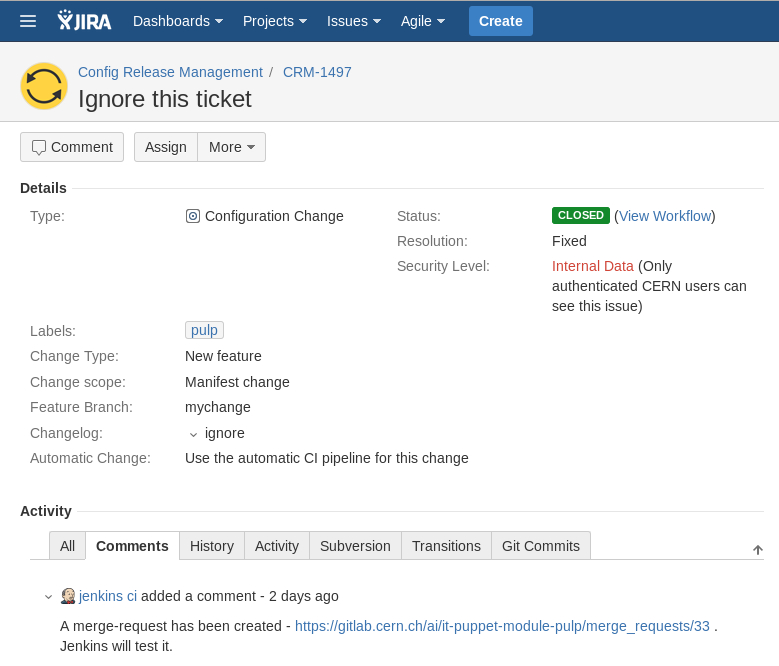
\includegraphics[width=\textwidth,height=\textheight,keepaspectratio]{ContinuousIntegrationWithJenkins/images/add_crm_change.jpg}
\caption{JIRA ticket to propose a new configuration change}
\end{figure}

When the user opens the ticket, the procedure is started, from now on the
whole work flow is automated and does not need any user interaction
(except, obviously, in case of tests failures).

Aidoctor, as described in the previous sections contains a script that
monitors the Jira service for new tickets. When the user creates a new
ticket this script forges a merge request on Gitlab using the ticket's
title and description, from the specified branch to the QA branch. The
link of the merge request is then posted in Jira to let the user have the
possibility to keep track of the work flow.

Jenkins monitors the Gitlab instance for new merge requests assigned to
the \textit{Jenkins CI} user, in fact we do not want our CI to take care
of all the merge requests. Whenever a new merge request is opened and the
assigner corresponds to the user associated with Jenkins a new build is
triggered. This means as well that users can test their changes using
the Continuous Integration infrastructure even without opening a CRM, but
simply assigning the merge request to Jenkins.

At this point Jenkins starts building the job called
\textit{it-puppet-module-modulename} with the parameters obtained from the
merge request. This job, that has been created in the previous sections
while adding the sample tests, consists in a set of sub-jobs:

\begin{enumerate}

  \item create-env

  Using as default QA. Overrides the module taken into consideration with
  the branch involved in the merge request.

  \item create-verify

  Selects a random machine from the corresponding pool and moves it to the
  new custom environment. Runs all the tests, both internal and external,
  and reports the results.

  \item destroy-vm

  The virtual machine just used is destroyed.

  \item destroy-env

  The custom environment is deleted.

\end{enumerate}

When the multi job is completed we can face two possible scenarios: in the
first option everything went smoothly, all the tests passed, the machine
has been build correctly and the user is happy with the result of its
change. In this case the merge request is automatically approved by
Jenkins and the change is merged in the QA branch. All the machines in the
environment QA will apply the change and all the service managers will
receive an email with a summary of the ongoing change.

On the other hand, if the tests fail the user has two options to proceed,
based on the nature of the errors. If the committed change is effectively
breaking the tests, it can fix the code simply pushing a new commit to the
custom branch containing the change. Jenkins will notice a new commit in
the branch and will test it again.

If the error has been generated by Jenkins or by a temporary malfunction,
and we want to test the same change again, all the user has to do is to
add a new comment to the merge request with "Please test". Even in this
case Jenkins will pick the change and run all the tests again.

\begin{figure}[H]
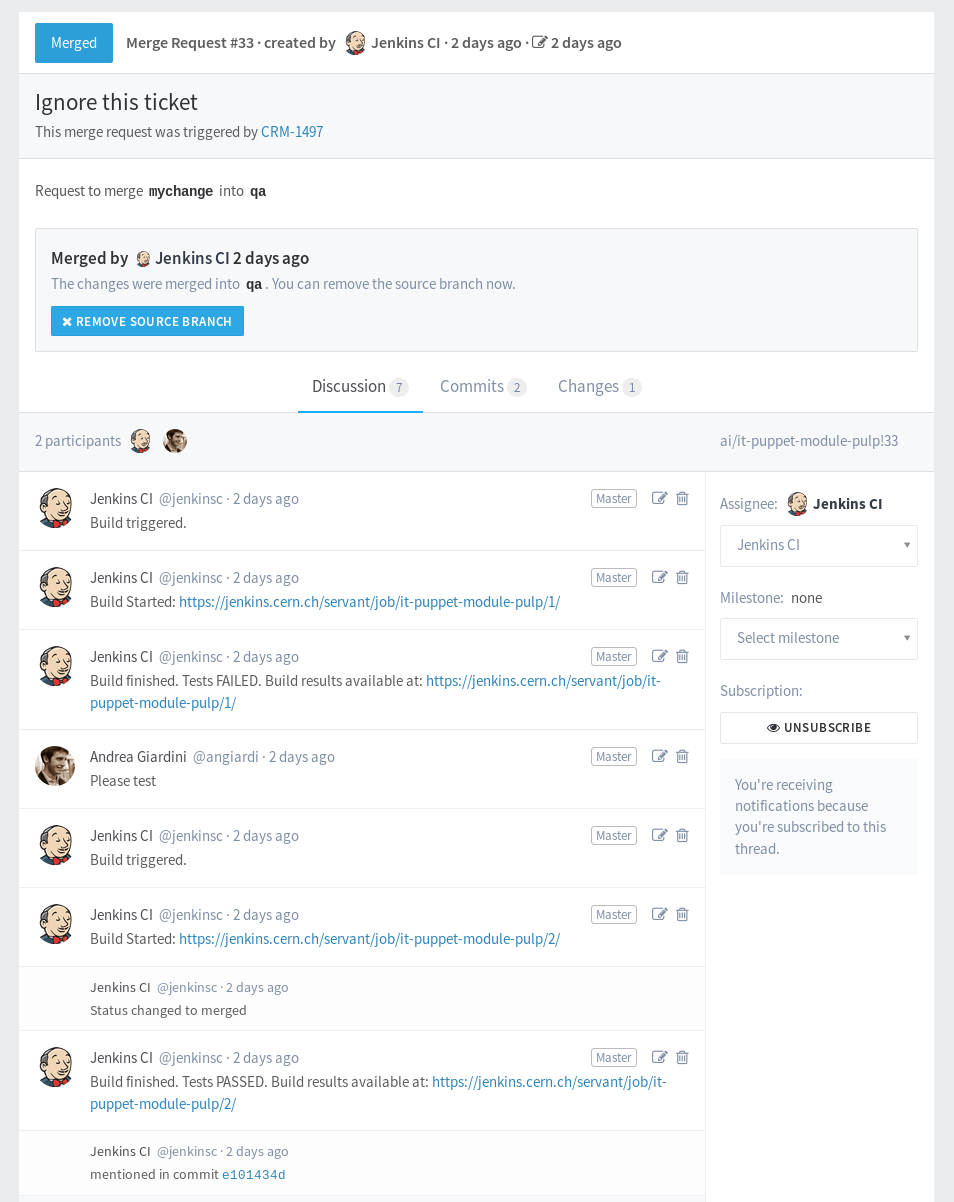
\includegraphics[width=\textwidth,height=\textheight,keepaspectratio]{ContinuousIntegrationWithJenkins/images/gitlab_merge_to_qa.jpg}
\caption{Gitlab merge request}
\end{figure}

After one week in the QA branch, if nobody had problem with the change,
Aidoctor creates a new merge request to move the change to production.

It is important to notice that, during the whole testing, the user does not
need to open the web interface of Jenkins except in case of errors. This was
indeed the aim of the project: simplify the testing procedure, adding
automation in a non-invasive way. Users do not need to learn a new software or
study how to get their own Jenkins instance up and running: a unified procedure
takes care of all the needs of the user and, after following a short
configuration guide, the team is ready to automate their deployments.
